\section{Methodology}\label{sec:methods}
\subsection{Research design}
The study is a quantitative simulation organised by the six phases of the Cross-Industry Standard Process for Data Mining (CRISP-DM)~\cite{chapman} (Figure~\ref{fig:design}). Decisions are weekly and walk-forward (Section~\ref{sec:model}), and all strategies share one optimiser, constraints and costs, so differences come from how sentiment enters the decision. All choices were made on the validation period, 2012--2014, then fixed with a cryptographic hash of the code and settings before the test period, January 2015 to December 2025 (\Weeks{} weeks), was run once (Figure~\ref{fig:timeline}).
\end{multicols}
\begin{figure}[H]\centering
\begin{tikzpicture}[node distance=2.2mm, every node/.style={font=\scriptsize, align=center},
  phase/.style={draw, rounded corners=1pt, text width=19.4mm, minimum height=14mm, fill=blue!5,
    execute at begin node={\hyphenpenalty=10000\relax}},
  arr/.style={-{Stealth[length=1.8mm]}, thick}]
\node[phase] (b) {\textbf{Business}\\\textbf{understanding}\\problem, questions, KPIs\\(Section~\ref{sec:intro})};
\node[phase, right=of b] (d) {\textbf{Data}\\\textbf{understanding}\\universe, prices, headlines\\(Section~\ref{sec:data})};
\node[phase, right=of d] (p) {\textbf{Data}\\\textbf{preparation}\\filters, FinBERT, gauge\\(Sections~\ref{sec:prep},~\ref{sec:gauge})};
\node[phase, right=of p] (m) {\textbf{Modeling}\\forecasts, optimiser, validation\\(Section~\ref{sec:methods})};
\node[phase, right=of m] (e) {\textbf{Evaluation}\\single test 2015--2025\\(Sections~\ref{sec:results},~\ref{sec:analysis})};
\node[phase, dashed, fill=white, right=of e] (u) {\textbf{Deployment}\\weekly batch job\\(Section~\ref{sec:implications})};
\draw[arr] (b)--(d); \draw[arr] (d)--(p); \draw[arr] (p)--(m); \draw[arr] (m)--(e); \draw[arr, dashed] (e)--(u);
\end{tikzpicture}
\caption{Research design following the six CRISP-DM phases~\cite{chapman}, with the sections that cover each phase. Deployment is discussed but not carried out (dashed).}\label{fig:design}
\end{figure}
\begin{figure}[H]\centering
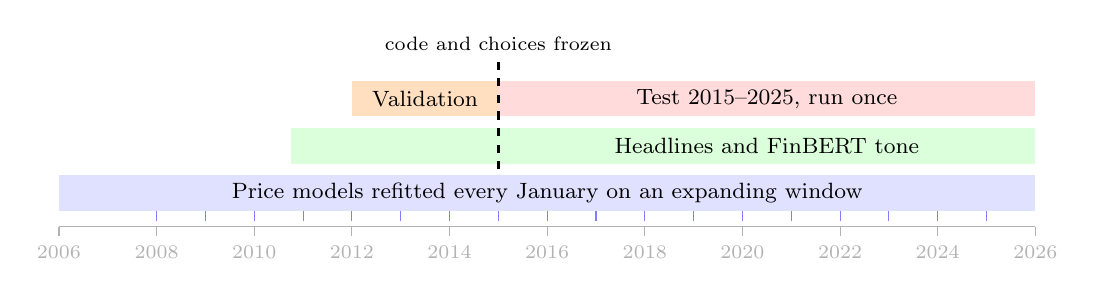
\begin{tikzpicture}[x=6.2mm, y=5mm, every node/.style={font=\footnotesize}]
\foreach \yr in {2006,2008,...,2026} {\draw[gray!60] (\yr-2005,0) -- (\yr-2005,-0.25) node[below, font=\scriptsize] {\yr};}
\draw[gray!60] (1,0) -- (21,0);
\fill[blue!12] (1,0.4) rectangle (21,1.3); \node at (11,0.85) {Price models refitted every January on an expanding window};
\fill[green!14] (5.75,1.6) rectangle (21,2.5); \node at (15.5,2.05) {Headlines and FinBERT tone};
\fill[orange!25] (7,2.8) rectangle (10,3.7); \node at (8.5,3.25) {Validation};
\fill[red!14] (10,2.8) rectangle (21,3.7); \node at (15.5,3.25) {Test 2015--2025, run once};
\draw[very thick, dashed] (10,1.45) -- (10,4.2) node[above, font=\scriptsize] {code and choices frozen};
\foreach \yr in {2008,...,2025} {\draw[blue!50] (\yr-2005,0.4) -- (\yr-2005,0.15);}
\end{tikzpicture}
\caption{Walk-forward timeline. Models are refitted every January (ticks) on data known before the first decision of the year; all choices are fixed on 2012--2014 before the test.}\label{fig:timeline}
\end{figure}
\begin{multicols}{2}

\subsection{Price forecasting models}
Six candidates represent these families: Ridge regression as the linear baseline~\cite{hoerl}, ARIMA per stock (order chosen by AIC), the factor composite, a random forest, gradient-boosted trees and an LSTM on the last eight weeks of inputs. The learning models use ten price and trading predictors (Table~\ref{tab:features}), ranked across stocks every week, and forecast returns relative to the cross-sectional mean. Fundamentals are not used because free point-in-time accounting data are unavailable for European firms. All models are pooled across stocks and refitted every January. The candidate with the highest mean weekly rank IC in the validation period is selected.
\end{multicols}
\begin{table}[H]\centering\footnotesize
\begin{tabularx}{\textwidth}{>{\raggedright\arraybackslash}p{29mm}>{\raggedright\arraybackslash}X}\toprule
Group & Inputs (values known at the decision cutoff)\\\midrule
Price (7) & 12-month momentum excluding the last month; 1-month and 1-week reversal; 60-day volatility; largest daily return over 20 days; beta to the universe over 52 weeks; distance to the 52-week high\\
Trading activity (3) & 20-day dollar volume; illiquidity (mean absolute daily return per dollar traded); abnormal volume (20-day versus 120-day dollar volume)\\
Sentiment & abnormal firm tone and abnormal sector tone (Eq.~\ref{eq:abnormal}), smoothed into the gauge\\\bottomrule
\end{tabularx}
\caption{Model inputs. Headline counts enter only through the shrinkage in Eq.~(\ref{eq:abnormal}).}\label{tab:features}
\end{table}
\begin{multicols}{2}

\subsection{Sentiment gauge}\label{sec:gauge}
The gauge combines the smoothed firm and sector scores, $G = [(1 - w)\, M^{f} + w\, M^{s}] / \mathrm{s.d.}$, where the firm-only ($w = 0$) and sector-only ($w = 1$) versions are $G^{f}$ and $G^{s}$. Validation chose between $w = 0$ and $w = 0.5$ by the larger absolute IC, and the sign of that IC decides whether the gauge is used for continuation or reversal. The s.d.\ is pooled across firms over the previous 52 weeks, which keeps the bands comparable as coverage grows. A view opens at $|G| \ge 1.5$ and closes below $|G| = 0.5$ (Figure~\ref{fig:gauge}).
\end{multicols}
\begin{figure}[H]\centering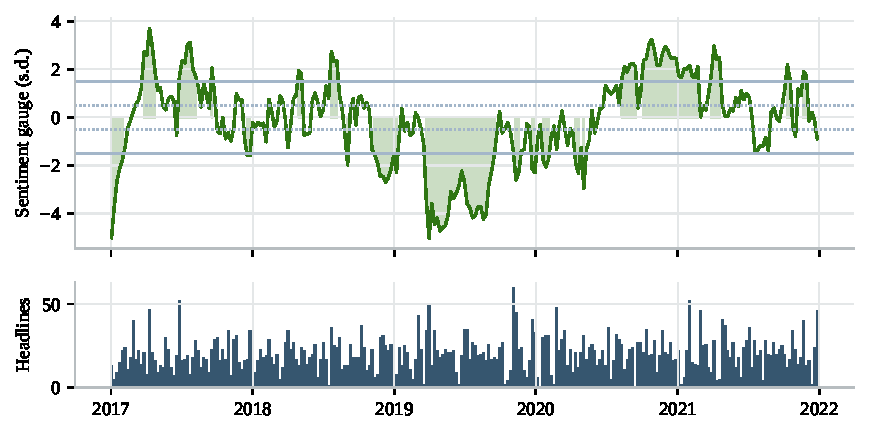
\includegraphics[width=\textwidth]{gauge_example}
\caption{Sentiment gauge and weekly headlines for Boeing, 2017--2021. Solid lines mark the entry bands and dotted lines the exit bands; shaded areas are weeks with the gauge beyond the entry band.}\label{fig:gauge}\end{figure}
\begin{multicols}{2}

\subsection{Sentiment as confirmation of the price forecast}
The selected price forecast is first converted into an expected relative return $\hat y^{P}$ by a regression through the origin of realised relative returns on the forecast over the previous three years. A Ridge model then learns how sentiment corrects the forecast. To avoid look-ahead, it is trained only on \emph{out-of-sample} errors $e = y - \hat y^{P}$, from forecasts made with earlier data, and is refitted every January:
\begin{equation}\label{eq:correction}
\begin{aligned}
\hat y^{C}_{i,t} &= \hat y^{P}_{i,t} + \beta_0 + \boldsymbol\beta^{\top} \mathbf x_{i,t} ,\\[2pt]
\mathbf x_{i,t} &= \bigl(\mathbf g_{i,t} ,\; d_{i,t}\, \mathbf g_{i,t}\bigr) ,\\[2pt]
\mathbf g_{i,t} &= \bigl(G^{f} ,\, G^{s} ,\, a^{f} ,\, a^{s}\bigr)_{i,t} ,
\end{aligned}
\end{equation}
where $G^{f}$ and $G^{s}$ are the firm and sector gauges, $a^{f}$ and $a^{s}$ the current week's abnormal firm and sector tone (Eq.~\ref{eq:abnormal}), and $d_{i,t} = \pm 1$ the direction of the price forecast; a simpler version without the weekly tone was rejected on validation. The agreement terms $d\,\mathbf g$ let sentiment strengthen a price signal it confirms and weaken, or overturn, one it contradicts. The Ridge penalty is chosen by generalised cross-validation~\cite{hoerl}.

\subsection{Optimisation model}\label{sec:model}
All optimised strategies solve the same problem every week (Table~\ref{tab:model}). The decision variables are the weights $\mathbf w$ of the $N_t$ investable stocks, which solve
\begin{equation}\label{eq:optimiser}
\begin{aligned}
\max_{\mathbf w}\;\; &\underbrace{\boldsymbol\mu^{\top} \mathbf w}_{\text{return}} \;-\; \underbrace{\frac{\delta}{2}\, \mathbf w^{\top} \boldsymbol\Sigma\, \mathbf w}_{\text{risk}} \;-\; \underbrace{\frac{c}{H} \sum_i \lvert w_i - \tilde w_i \rvert}_{\text{trading cost}}\\[4pt]
\text{s.t.}\;\; &\textstyle\sum_i w_i = 1 , \qquad 0 \le w_i \le 0.05 \quad \forall i ,
\end{aligned}
\end{equation}
a convex quadratic programme, where $\tilde{\mathbf w}$ are last week's weights after price drift. A trade is paid once but earns over several weeks, so its cost $c$ is spread over the expected holding time $H$.

The expected returns $\boldsymbol\mu$ are the Black--Litterman posterior around the reference portfolio, equal weighting. Its implied returns $\boldsymbol\pi = \delta \boldsymbol\Sigma\, \mathbf w_{\mathrm{EW}}$ make $\mathbf w_{\mathrm{EW}}$ optimal when there are no views and no costs. A view states that stock $i$ will beat $\pi_i$ by $\alpha_i = \widehat{\mathrm{IC}}_t\, \sigma_i\, z_i$, where $\sigma_i$ is its weekly volatility and $z_i$ the signal in standard deviations. With prior uncertainty $\tau\boldsymbol\Sigma$ and view uncertainty $\boldsymbol\Omega = \tau \mathbf D_S$~\cite{blacklitterman,helitterman}, $\tau$ cancels:
\begin{equation}\label{eq:bl}
\boldsymbol\mu = \boldsymbol\pi + \boldsymbol\Sigma_{\cdot S} \bigl(\boldsymbol\Sigma_{SS} + \mathbf D_S\bigr)^{-1} \boldsymbol\alpha_S ,
\end{equation}
where $S$ is the set of stocks with views, $\boldsymbol\Sigma_{\cdot S}$ the covariance of all stocks with them and $\mathbf D_S$ their variances.

The \emph{confidence} in a view enters through $\boldsymbol\Omega$, which makes each view as uncertain as the stock's own return in the prior, so a single uncorrelated view moves $\mu_i$ halfway from $\pi_i$ to $\pi_i + \alpha_i$. The size of the view follows the signal's record, as $\widehat{\mathrm{IC}}_t$ is its mean weekly rank IC over the previous three years, set to zero if negative or if fewer than 52 weeks are known, so a signal without measured skill has no views.

The strategies differ only in their views: \emph{price only} (all stocks; $z$ is the cross-sectional z-score of the price forecast), \emph{price + sentiment} (all stocks; Eq.~\ref{eq:correction}) and \emph{sentiment-driven} (only stocks with an open gauge view; $z = G$, capped at $\pm 3$). \emph{Minimum variance} solves Eq.~(\ref{eq:optimiser}) with $\boldsymbol\mu = \mathbf 0$. Benchmarks are equal weighting, rebalanced weekly, and buy-and-hold URTH. The rebalancing rule is the same every week:
\begin{enumerate}
\item At the cut-off, Thursday 22:00 UTC after the U.S. close, form the investable set (stocks with at least 40 of the last 52 weekly returns), $\boldsymbol\Sigma$, the signals and $\widehat{\mathrm{IC}}_t$ from data published before it.
\item Compute $\boldsymbol\mu$ (Eq.~\ref{eq:bl}) and solve Eq.~(\ref{eq:optimiser}) from $\tilde{\mathbf w}$.
\item Trade to the solution at each stock's Friday close, selling stocks that leave the universe, and pay $c \sum_i |w_i - \tilde w_i|$.
\item Hold for one week; the drifted weights become $\tilde{\mathbf w}$.
\end{enumerate}
\end{multicols}
\begin{table}[H]\centering\footnotesize
\begin{tabularx}{\textwidth}{>{\raggedright\arraybackslash}p{30mm}>{\raggedright\arraybackslash}X>{\raggedright\arraybackslash}p{36mm}}\toprule
Element & Specification & Setting\\\midrule
Decision variables & Weight $w_i$ of each investable stock after the weekly trade & $N_t$ = 140--141 stocks\\
Objective & Maximise expected return minus risk and trading-cost penalties, Eq.~(\ref{eq:optimiser}) & --\\
Risk term & $\frac{\delta}{2}\mathbf w^{\top}\boldsymbol\Sigma\mathbf w$; Ledoit--Wolf covariance of the last 52 weekly USD returns~\cite{ledoitwolf} & $\delta=2.5$\\
Trading-cost term & $\frac{c}{H}\sum_i|w_i-\tilde w_i|$ from the drifted weights $\tilde{\mathbf w}$ & $c=10$ bp, $H=4$ weeks\\
Reference portfolio & Equal weight; implied returns $\boldsymbol\pi=\delta\boldsymbol\Sigma\mathbf w_{\mathrm{EW}}$ & $w_i=1/N_t$\\
Expected returns & Black--Litterman posterior, Eq.~(\ref{eq:bl}) & $\tau$ cancels\\
Views & $\alpha_i=\widehat{\mathrm{IC}}_t\,\sigma_i\,z_i$ on the stocks in $S$ & gauge capped at $\pm3$\\
View confidence & $\boldsymbol\Omega=\tau\,\mathrm{diag}(\boldsymbol\Sigma_{SS})$; view size scaled by the trailing IC & 3-year IC, $\ge$52 weeks, floored at 0\\
Constraints & Fully invested, long-only, issuer limit (UCITS 5\%); no leverage, cash or sector limits & $\sum_i w_i=1$, $0\le w_i\le0.05$\\
Rebalancing & Decide Thursday 22:00 UTC, trade at each stock's Friday close, hold one week & \Weeks{} weekly decisions\\
Solver & Convex quadratic programme & Clarabel (cvxpy)\\\bottomrule
\end{tabularx}
\caption{Specification of the optimisation model shared by all optimised strategies; minimum variance sets $\boldsymbol\mu=\mathbf 0$.}\label{tab:model}
\end{table}
\begin{multicols}{2}

\subsection{Costs and evaluation}
Every purchase and sale costs $c = 10$ basis points of traded value, close to the measured costs of large institutional trades~\cite{frazzini}; 0, 5 and 20 basis points are tested. KPIs are compound annual growth (CAGR), volatility, the Sharpe and Sortino ratios (Treasury yield as risk-free rate), maximum drawdown, turnover and cost. Differences between strategies get 95\% intervals from a paired bootstrap that resamples 13-week blocks to keep autocorrelation (2,000 draws)~\cite{politis}; mean ICs and alphas use Newey--West (HAC) standard errors~\cite{neweywest}. RQ1 is tested with an event study of daily returns relative to the stock's regional average around tradable gauge signals, and with Fama--MacBeth regressions of next-week returns on the gauges with and without price controls~\cite{famamacbeth}. Robustness tests change one setting at a time. Table~\ref{tab:decisions}, Figure~\ref{fig:mechanism}, Section~\ref{sec:coverage} and Appendix~\ref{app:fnspid} report analyses added after the test; they use the frozen models and change no choice.
